%!TEX root = ../msc_thesis.tex

\chapter{Active Learning}
\label{ch:active_learning}

%%%%%%%%%%%%%%%%%%%%%%%%%%%%%%%%%%%%%%%%%%%%%%%%%%%%%%%%%%%%%%%%%%%%%%%%%%%%%%%%%%%%%%%%%%
%%%%%%%%%%%%%%%%%%%%%%%%%%%%%%%%%%%%%%%%%%%%%%%%%%%%%%%%%%%%%%%%%%%%%%%%%%%%%%%%%%%%%%%%%%
%%% AL
%%%%%%%%%%%%%%%%%%%%%%%%%%%%%%%%%%%%%%%%%%%%%%%%%%%%%%%%%%%%%%%%%%%%%%%%%%%%%%%%%%%%%%%%%%
%%%%%%%%%%%%%%%%%%%%%%%%%%%%%%%%%%%%%%%%%%%%%%%%%%%%%%%%%%%%%%%%%%%%%%%%%%%%%%%%%%%%%%%%%%

% \section{Active Learning}

An active learning problem is one in which the learner selects its own training data. For example, in a supervised learning problem where we are given a data set with features $\boldsymbol{X}$ and response variable $\boldsymbol{y}$. First we train a model $\hat{f}$ with the data that we have, afterwards the learner can choose new data $\boldsymbol{x}^*$ from an unlabeled pool of data, ask to an \textit{oracle} what the corresponding output $y^*$ is, and then add the pair $(\boldsymbol{x}^*, {y}^*)$ to the training data. The main goal of active learning is to select which $\boldsymbol{x}^*$ to incorporate to the training data \cite{cohn1996active}.

The new example is chosen using an \textbf{acquisition function} $a(x, \hat{f})$ that is usually based on the model's uncertainty about the prediction. The new observation $\boldsymbol{x}^*$ is chosen so that it maximizes the acquisition function of all the observations in the pool set. In practice, the oracle is usually a human that gives the corresponding label ${y}^*$. After the new observation is added to the training data, the model is retrained with the updated data set. This process is iteratively repeated, with the training set increasing in size with every iteration. In the end, it is expected that this procedure leads to a better predictive performance than randomly selecting new observations to add to the training data.

The acquisition functions that will be used and compared in this work are four, and three of them use the posterior predictive distribution, particularly, the posterior predictive probability of an observation $\boldsymbol{x}^*$ having a label $y^*$ belonging to a class $c$, denoted as  $p(y^* = c | \boldsymbol{X}, \boldsymbol{y}, \boldsymbol{x}^*)$. Naturally, because of the definition of these acquisition functions, they only work in classification problems.

\begin{enumerate}
  \item Predictive entropy:

  $ \mathbb{H} \left[ y^* | \boldsymbol{X}, \boldsymbol{y}, \boldsymbol{x}^* \right] = - \sum_c p(y^* = c | \boldsymbol{X}, \boldsymbol{y}, \boldsymbol{x}^*) \log p(y^* = c | \boldsymbol{X}, \boldsymbol{y}, \boldsymbol{x}^*)$.

  \item Bayesian Active Learning by Disagreement (BALD):

  $ \mathbb{H} \left[ y^* | \boldsymbol{X}, \boldsymbol{y}, \boldsymbol{x}^* \right] - \mathbb{E}_{p(\boldsymbol{\theta} | \boldsymbol{X}, \boldsymbol{y})} \left[ \mathbb{H} \left[ y^* | \boldsymbol{x}^*, \boldsymbol{\theta} \right] \right]$.

  \item Variation ratios: $1 - \max_y p(y^* | \boldsymbol{X}, \boldsymbol{y}, \boldsymbol{x}^*)$.

  \item Random: Choosing an observation uniformly random from the pool of unlabeled data.

\end{enumerate}



\begin{figure}[H]
    \centering
    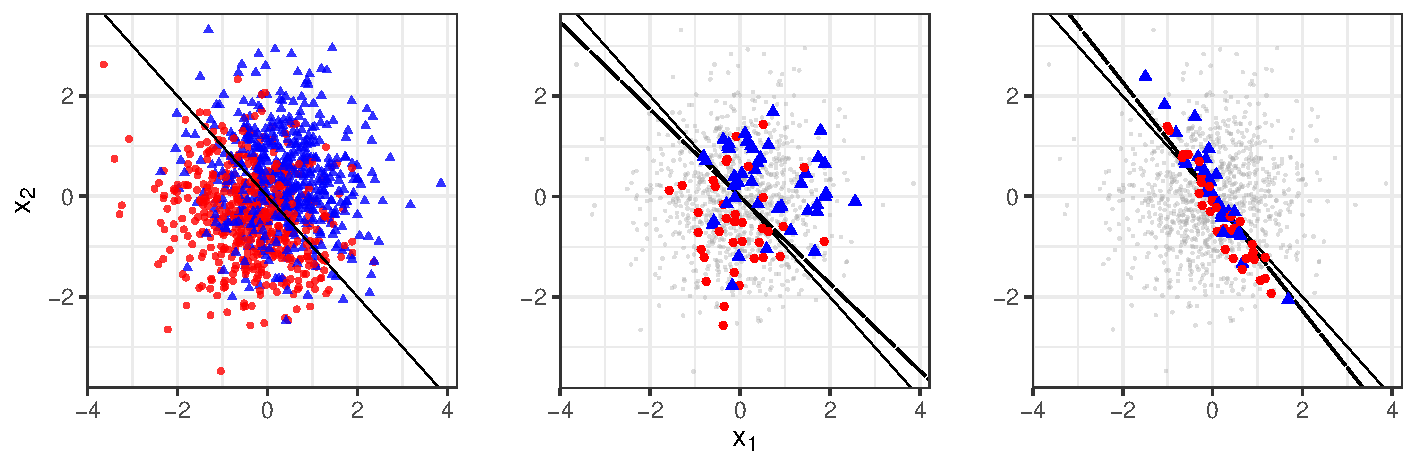
\includegraphics[width=\textwidth]{log_reg_AL_decision_boundary_plot}
    \caption{AL example 1.}
    \label{fig:log_reg_AL_decision_boundary_plot}
\end{figure}



\begin{figure}[H]
    \centering
    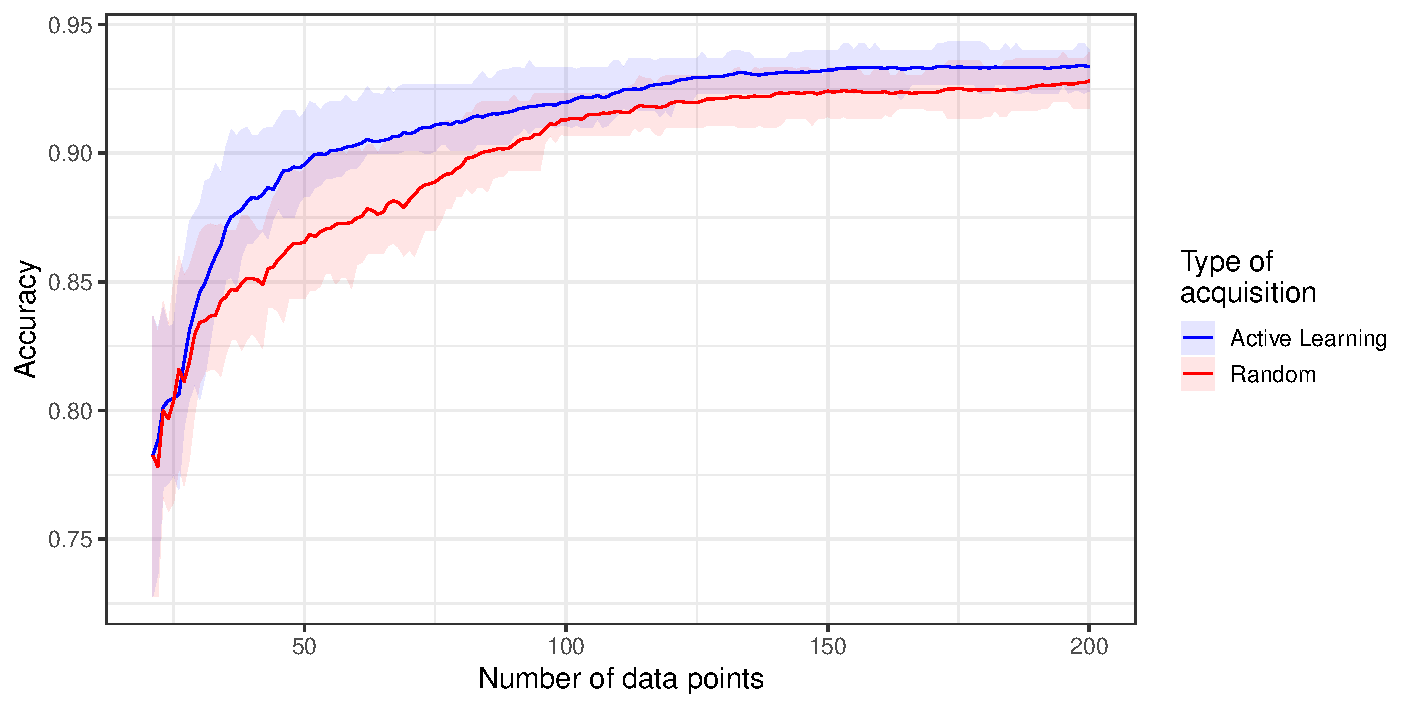
\includegraphics[width=\textwidth]{log_reg_AL_accuracies_plot}
    \caption{AL example 1.}
    \label{fig:log_reg_AL_accuracies_plot}
\end{figure}
